\documentclass[11pt, a4paper]{article}
% \usepackage[T1]{fontenc}
\usepackage[utf8]{inputenc}
\usepackage{listings}
\usepackage[margin=1.0in]{geometry}
\usepackage{color}
\usepackage{graphicx}
\usepackage{tabularx}
\usepackage{url}
\usepackage{float}
\usepackage{enumitem}
\usepackage{subcaption}

\lstnewenvironment{python}[1][]
{\lstset{
		language=python,
		numbers=left,
		numberstyle=\tiny,
		keywordstyle=\color{blue},       	% keyword style
		basicstyle=\footnotesize\ttfamily,	% font
		numbers=left,						% line numbers
		tabsize=2,							% tabsize in spaces
		#1}}
{}

\lstnewenvironment{bash}[1][]
{\lstset{
		language=bash,
		numbers=left,
		numberstyle=\tiny,
		numbers=none,
		basicstyle=\footnotesize\ttfamily,	% font
		tabsize=2,							% tabsize in spaces
		#1}}
{}

\lstnewenvironment{code}[1][]
{\lstset{numbers=left,
		numberstyle=\tiny,
		keywordstyle=\color{blue},       % keyword style
		basicstyle=\footnotesize\ttfamily,	% font
		numbers=left,						% line numbers
		tabsize=2,							% tabsize in spaces
		#1}}
{}

\title{DezSys05 - Load Balancing}
\author{Elias Frantar, Gary Ye (5AHITT)}
\date{\today{}, Wien}
\begin{document}

\lstset{
  backgroundcolor=\color{white},   % choose the background color; you must add \usepackage{color} or \usepackage{xcolor}
  basicstyle=\footnotesize,        % the size of the fonts that are used for the code
  breakatwhitespace=false,         % sets if automatic breaks should only happen at whitespace
  breaklines=true,                 % sets automatic line breaking
  captionpos=b,                    % sets the caption-position to bottom
% commentstyle=\color{mygreen},    % comment style
  deletekeywords={...},            % if you want to delete keywords from the given language
  escapeinside={\%*}{*)},          % if you want to add LaTeX within your code
  extendedchars=true,              % lets you use non-ASCII characters; for 8-bits encodings only, does not work with UTF-8
% frame=single,                    % adds a frame around the code
  keepspaces=true,                 % keeps spaces in text, useful for keeping indentation of code (possibly needs columns=flexible)
  keywordstyle=\color{blue},       % keyword style
% language=bash,                   % the language of the code
  morekeywords={*,...},            % if you want to add more keywords to the set
  numbers=none,                    % where to put the line-numbers; possible values are (none, left, right)
  numbersep=5pt,                   % how far the line-numbers are from the code
%  numberstyle=\tiny\color{gray}, % the style that is used for the line-numbers
  rulecolor=\color{black},         % if not set, the frame-color may be changed on line-breaks within not-black text (e.g. comments (green here))
  showspaces=false,                % show spaces everywhere adding particular underscores; it overrides 'showstringspaces'
  showstringspaces=false,          % underline spaces within strings only
  showtabs=false,                  % show tabs within strings adding particular underscores
%  stepnumber=1,                    % the step between two line-numbers. If it's 1, each line will be numbered
  stringstyle=\color{red},     % string literal style
  tabsize=2,                       % sets default tabsize to 2 spaces
  title=\lstname,                   % show the filename of files included with \lstinputlisting; also try caption instead of title
  belowskip=-3em,    
}

\setlength\parindent{0pt}

\maketitle
\newpage
\tableofcontents
\newpage

\section{Requirements}

\subsection{Aufgabenstellung}

Es soll ein Load Balancer mit mindestens 2 unterschiedlichen
Load-Balancing Methoden (jeweils 7 Punkte) implementiert werden
(ähnlich dem PI Beispiel [1]; Loesung zum Teil veraltet [2]). Eine
Kombination von mehreren Methoden ist moeglich. Die Berechnung
bzw. das Service ist frei waehlbar!
\\\\
Folgende Load Balancing Methoden stehen zur Auswahl:

\begin{itemize}
	\item Weighted Round-Robin
	\item Least Connection
	\item Least Connected Slow- Start Time
	\item Weighted Least Connection
	\item Agent Based Adaptive Balancing / Server Probes
\end{itemize}

Um die Komplexitaet zu steigern, soll zusaetzlich eine "Session
Persistence" (2 Punkte) implementiert werden.

\subsection{Auslastung}
Es sollen die einzelnen Server-Instanzen in folgenden Punkten belastet werden können:

\begin{itemize}
	\item Memory (RAM)
	\item CPU Cycles
	\item I/O Zugriff (Harddisk)
\end{itemize}

Bedenken Sie dabei, dass die einzelnen Load Balancing Methoden unterschiedlich auf diese Auslastung reagieren werden. Dokumentieren Sie dabei aufkommenden Probleme ausführlich.

\subsection{Tests}

Die Tests sollen so aufgebaut sein, dass in der Gruppe jedes Mitglied
mehrere Server fahren und ein Gruppenmitglied mehrere Anfragen an den
Load Balancer stellen. Fuer die Abnahme wird empfohlen, dass jeder
Server eine Ausgabe mit entsprechenden Informationen ausgibt, damit
die Verteilung der Anfragen demonstriert werden kann.

\subsection{Modalitaeten}

Gruppenarbeit: 2 Personen Abgabe: Protokoll mit Designueberlegungen /
Umsetzung / Testszenarien, Sourcecode (mit allen notwendigen
Bibliotheken), Java-Doc, Jar

\subsection{Quellen}

[1] "Praktische Arbeit 2 zur Vorlesung 'Verteilte Systeme' ETH
Zuerich, SS 2002", Prof.Dr.B.Plattner, Uebernommen von
Prof.Dr.F.Mattern

(http://www.tik.ee.ethz.ch/tik/education/lectures/VS/SS02/Praktikum/aufgabe2.pdf)

[2] http://www.tik.ee.ethz.ch/education/lectures/VS/SS02/Praktikum/loesung2.zip

\newpage

\section{Effort Estimation and Work Distribution}

The following table compares the estimated with the actually needed
amount of time for completing each individual task.
\\\\
The estimation is in the second column while the columns that follow
are actual values.

\parskip 12pt
\begin{tabular} {| l | c | c | c | c |}
	\hline
	Task					&	Estimation		& 	Elias 	& 	Gary 	& 	Team	\\ \hline \hline
	Preparation				&	2				&	0.5		&  	0.5		&	1		\\ \hline
	Design					&	4				&	2		&	2		&	4		\\ \hline
	Implementation			&	6				&	5		&	5		& 	10 		\\ \hline
	Testing					&	4				&	2		& 	2		& 	4 		\\ \hline
	Documentation			&	10				&	6		&	4		& 	8		\\ \hline 
	Total					&	26				&	15.5	&	13.5	& 	29		\\
	\hline
\end{tabular}

\section{Design}

\subsection{Assumptions}

Because of the limited time for the present exercise, it is not
possible to handle all problems. Therefore the following assumptions
have been made under which our solution will work:

\vspace{-10pt}
\begin{itemize}
\item Servers are registered at the load-balancer before and only
  before startup
\item Sessions cannot end (except if the associated server goes down)
\item All connections have the same size/weight/package-length/...
\end{itemize}
\vspace{-10pt}

Deduced from these assumptions our implementation will have the
following functional restrictions:

\vspace{-10pt}
\begin{itemize}
\item Additional servers \textit{cannot} be dynamically added during
  runtime
\item Load-balancer will \textit{not} be acknowledged when a
  connection is closed
\item A client who connected to a server once will (session
  persistence) \textit{always} be reconnected to same server (as long
  as the load-balancer is up)
\item Load will only be balanced depending on \textit{the number of
    connections}, thus ignoring their length/weight/traffic/...
\end{itemize}
\vspace{-10pt}

Even though our program will not implement registering or unregistering additional servers during run-time, our design will take this feature into account. In addition the load-balancer will automatically unregister servers which failed to often, i.e. which went down.

\subsection{Technologies}

\subsubsection{Remote Procedure Call}

XML RPC is a technology that has already been thoroughly addressed in
the fourth grade of the IT department. Due to the preexisting
experience and the simpleness of this technology, we decided to use
the Xmlrpc library provided by Apache.

Its weakness in the performance, compared to other technologies, e.g.,
RMI, has not been a concern for us since this exercise is designed to
teach the different load balancing strategies. 

Apache's Java implementation of XML-RPC can be downloaded from \cite{xmlrpc-v3} (V3) or \cite{xmlrpc-v2} (V2).

\subsection{Load Balancing Scheduling Strategies}
\label{subsec:strategy}
From the given list of the scheduling strategies we picked Weighted
Round Robin and Least Connection First as the strategies to be
analyzed.

In the following sections we will, for simplicity's sake, abbreviate
Weighted Round Robin and Least Connection First as WRR and LCF
respectively.

Since the scheduling strategies that can be found in the Internet are
very abstract, we will also describe how we concretely applied them in
the use case of our application. 

\subsubsection{Weighted Round Robin}

\textit{WRR is not a standardized algorithm, and therefore there is no real definition on how it should "exactly" work. So we chose our own implementation, which is described below.}
\\\\
The WRR algorithm is an advancement of the primitive Round-Robin algorithm. RR always assigns the next connection to the next server and thereby evenly distributes the weight among all servers. WRR does essentially the same thing except that the weight will be distributed depending on preconfigured values.
\\\\
In detail every server has an attribute \lstinline|weight|, a relative number of the weight to assign to this server. The only thing that matters here is the relation to the other numbers. It does make no difference if two servers have both weight 100 or 1, they will get exactly the same amount of connections assigned.
\\\\
Thus the algorithm assigns connections to the servers in standard Round Robin fashion while incrementing connection-counters for every server until this counter is larger than the weight. In that case the server is skipped. This procedure continues until all servers are "full", then the counters are reset and the algorithm continues as usual.

\subsubsection{Least Connection First}

The LCF strategy can be explained very simply. For each server
instance $i$ we assign a number $c_i$, which denotes the number of
active/open connections on server $i$. Whenever the load balancer
receives a new request, it searches for the server with the minimum
$c_i$ and picks it as the server that should process the new
request. It subsequently increments $c_i$ by $1$. 

Denote $n$ as the number of servers that the load balancer
maintains. A simple algorithm iterates through all the given servers
and picks the server with the minimum $c_i$, which results in a linear
$O(n)$ algorithm. This might work well in practice, since $n$ cannot
range to more than 3 figures in reality (except large companies like
Google, NSA), but it is still theoretically slow. 

We can improve the searching step to $O(\log n)$ by using a subtle
data structure like a Balanced Binary Search Tree. Probably the
easiest BBST data structure to implement is a treap, which relies its
logarithmic height on the randomness of the priority keys.

\subsection{Software Design}

The following image shows the final submission design as a UML class-diagram.

\begin{figure}[H]
	\centering
	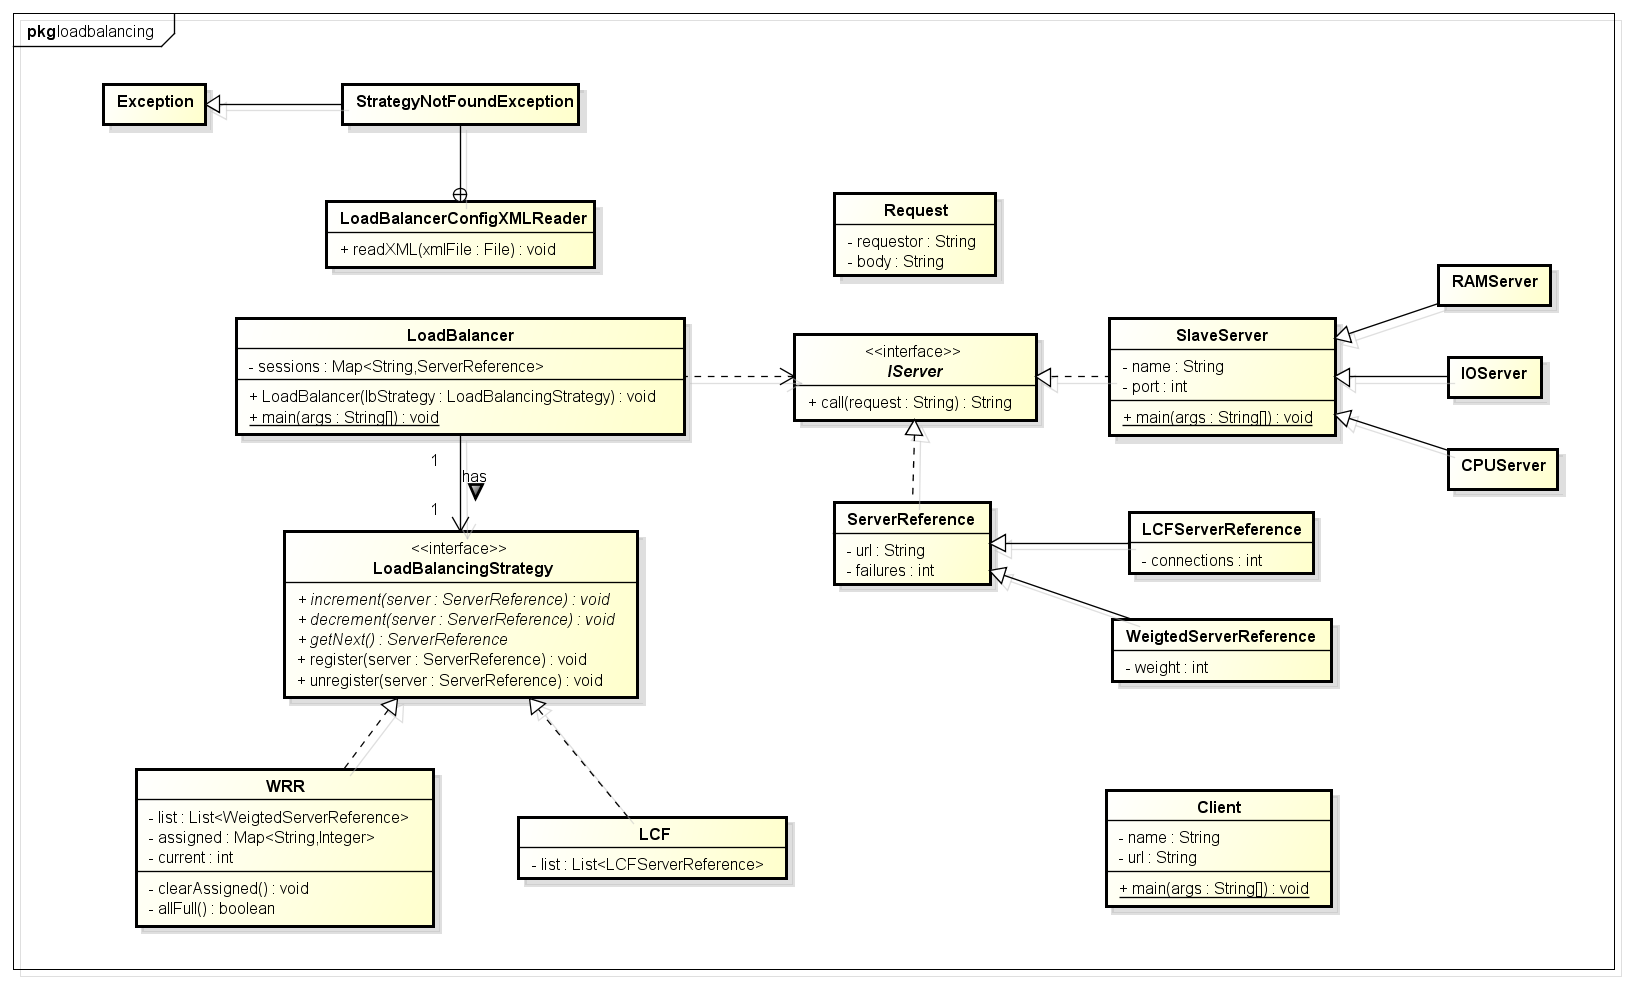
\includegraphics[width=\textwidth]{img/class-diagram}
	\caption{UML class diagram design}
\end{figure}

\section{Testing}

\subsection{Unit Testing}

The following show the results and coverage of our unit-tests.

\begin{figure}[H]
	\centering
	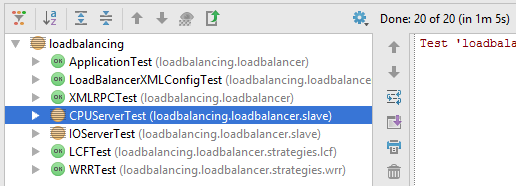
\includegraphics[height=1.5in]{img/tests}
	\caption{Unit-test results}
\end{figure}
\begin{figure}[H]
	\centering
	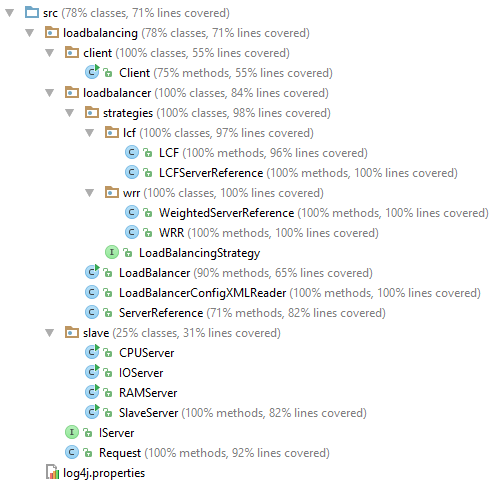
\includegraphics{img/coverage}
	\caption{Unit-test coverage}
\end{figure}

The strategies, which were mentioned in \ref{subsec:strategy}, were tested thoroughly with virtually 100 percentage code coverage.
For the load-balancer itself we performed some additional manual test described in the next section.

\subsection{Manual Testing}

For manual testing we performed the following action in order:

\begin{enumerate}
	\item started 2 \lstinline|SlaveServer|s by calling the with args \lstinline|9000 9001|
	\item started the \lstinline|LoadBalancer| with args \lstinline|5000 config.xml|
	\item started 3 clients with different names (with args \lstinline|client_name http://localhost:5000 Hello|)
\end{enumerate}

The following figures show the received console output of all 5 programs.

\begin{figure}[H]
	\centering
	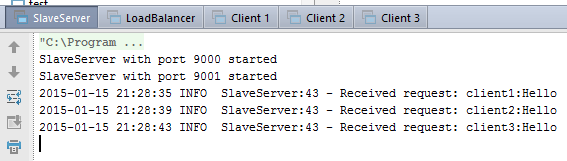
\includegraphics[height=1in]{img/test-servers}
	\caption{Console output of \lstinline|SlaveServer.java|}
\end{figure}
\begin{figure}[H]
	\centering
	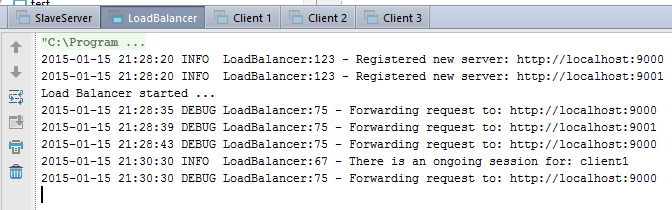
\includegraphics[height=1in]{img/test-loadbalancer}
	\caption{Console output of \lstinline|LoadBalancer.java|}
\end{figure}
\begin{figure}[H]
	\centering
	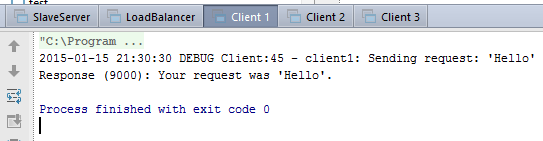
\includegraphics[height=1in]{img/test-client1}
	\caption{Console output of \lstinline|Client.java| (1)}
\end{figure}
\begin{figure}[H]
	\centering
	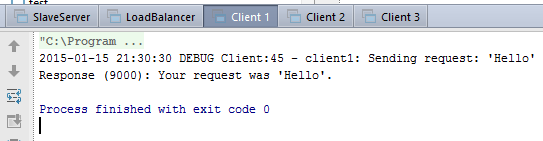
\includegraphics[height=1in]{img/test-client1}
	\caption{Console output of \lstinline|Client.java| (2)}
\end{figure}
\begin{figure}[H]
	\centering
	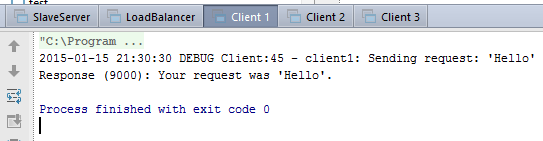
\includegraphics[height=1in]{img/test-client1}
	\caption{Console output of \lstinline|Client.java| (3)}
\end{figure}

One can easily observe in the output that Client 1 and Client 3 both received the response from the server on port 9000 whereas Client 2 received it from the server on port 9001, which means that the load-balancing worked properly.
\\\\
For testing the session persistance we simply restarted Client 1 to see if it gets the result from port 9000 and not from port 9001.

\begin{figure}[H]
	\centering
	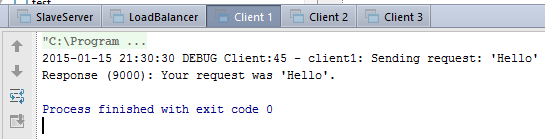
\includegraphics[height=1in]{img/test-session_persistance}
	\caption{Console output of \lstinline|Client.java| (1) when testing session-persistance}
\end{figure}

It worked as expected.
\\\\
\textit{Note that it doesn't make any difference for this test case if we start \lstinline|SlaveServers| or for example \lstinline|CPUServers|. We only chose the former since it returns responses that are easier to verify.}

\subsection{Load Tests}

Since our implemented algorithms are \textbf{completely independent} of the actual "load" of the servers, we did not expect any special results, i.e. the tests went exactly as described above.
\\\\
Not considering the \textit{real} load can of course be a major problem in real world applications. For example if a single server always gets the calls that require the most processing power, it might get overloaded. \textit{Therefore the difficulty of performing the tasks and the capacities of the servers should always be considered when implementing load balancers.}

\section{Occurred Problems}

\subsection{XML-RPC Default Constructor}

When making a remote procedure call on a class that has no default
constructor an Instantiation Exception will be thrown from the server.

This has been a nasty bug for an undefined time. 

\subsection{Wrong XML-RPC Version}

For some reason the newest version of XML-RPC behaved very strangely. Even after quite a lot fo research we were unable to register objects as servers, i.e. it was only possible to register classes from which XML-RPC automatically generates objects. Since we needed to register objects (for having servers with different ports) though we had to fix this serious problem.
\\\\
The solution was to downgrade to XML-RPC version 2. (Download: \cite{xmlrpc-v2}) There the desired registering could be performed with a single easy line of code:

\vspace{5pt}
\begin{lstlisting}
try {
    WebServer webServer = new WebServer(port);
    webServer.addHandler("Server", this);
    webServer.start();
} catch (Exception e) {
    System.out.print("Starting the server failed: " + e.getMessage());
}
\end{lstlisting}

\subsection{log4j.properties not found}

Another problem that occurred while working on the assignment, was that \lstinline|log4j| \cite{log} did not work properly, i.e. it was throwing around with some odd Exceptions even though we had already added a \lstinline|log4j.properties| file.
\\\\
It turned out that this file must not be in the project root-directory, but in the \lstinline|src/| folder. When fixing that everything worked fine again.

\subsection{log4j from ant}

When originally executing the program with the ant-buildfile it couldn't find the \lstinline|log4j.properties| file.
\\\\
This file can be specified via \lstinline|<sysproperty key="log4j.configuration" value="file:src/log4j.properties"/>| in an ant \lstinline|<java>| tag \cite{ant-log}.


\nocite{*}
\bibliographystyle{plain}
\bibliography{bibliography}

\end{document}
